\documentclass[xcolor=dvipsnames]{beamer}

\makeatletter

%HAY QUE ELEGIR EL QUE CORRESPONDA

%\usepackage{mathpazo}%Letra palatino con fuentes para matemáticas
\usepackage[T1]{fontenc}
\usepackage[utf8]{inputenc}
\usepackage{graphicx}
\usepackage{url}
\usepackage{amsmath}
\usepackage{booktabs}
\usepackage{textcomp}%%needed for the euro symbol

\date{}

\usepackage[emulate=units]{siunitx}
\sisetup{per=fraction, fraction=nice, decimalsymbol=comma}
\newunit{\wattpeak}{Wp}
\newunit{\watthour}{Wh}
\newunit{\amperehour}{Ah}

\setbeamercovered{transparent}
\setbeamertemplate{navigation symbols}{}
\usefonttheme{structuresmallcapsserif} 
\usefonttheme{serif} 
\usefonttheme{structurebold}

%\usepackage{epstopdf}


\usepackage[spanish]{babel}
\addto\shorthandsspanish{\spanishdeactivate{~<>}}

\hypersetup{pdfauthor={Oscar Perpi\~n\'an},%
    pdftitle={Energ\'ia Solar Fotovoltaica},%
    filecolor=blue,%
    urlcolor=blue}



%\usepackage{handoutWithNotes} %para hacer papel con notas 
%\pgfpagesuselayout{4 on 1 with notes}[a4paper,border shrink=5mm]



%\usepackage{pgfpages}
%\pgfpagesuselayout{2 on 1}[a4paper,border shrink=5mm]


%\usepackage{mathpazo}%Letra palatino con fuentes para matemáticas
\usepackage[T1]{fontenc}
\usepackage[utf8]{inputenc}
\usepackage{graphicx}
\usepackage{url}
\usepackage{amsmath}
\usepackage{booktabs}

\usepackage[spanish]{babel}
\addto\shorthandsspanish{\spanishdeactivate{~<>}}


\usepackage{hyperref}
% \hypersetup{pdfauthor={Oscar Perpi\~n\'an},%
%     pdftitle={Energ\'ia Solar Fotovoltaica},%
%     filecolor=blue,%
%     urlcolor=blue}

\hypersetup{
    bookmarks=true,         % show bookmarks bar?
%    unicode=true,          % non-Latin characters in Acrobat’s bookmarks
    bookmarksnumbered=false,
    bookmarksopen=false,
    breaklinks=true,
    backref=true,
    pdftoolbar=true,        % show Acrobat’s toolbar?
    pdfmenubar=true,        % show Acrobat’s menu?
    pdffitwindow=false,     % window fit to page when opened
    pdfstartview={FitH},    % fits the width of the page to the window
    pdftitle={Energía Solar Fotovoltaica},    % title
    pdfauthor={Oscar Perpiñán Lamigueiro},     % author
    pdfsubject={Electrotecnia},   % subject of the document
    pdfcreator={AucTeX/Emacs},   % creator of the document
    pdfproducer={LaTeX}, % producer of the document
    pdfnewwindow=true,      % links in new window
    pdfborder={0 0 0},
    colorlinks=true,       % false: boxed links; true: colored links
    linkcolor=,          % color of internal links
    citecolor=BrickRed,        % color of links to bibliography
    filecolor=black,      % color of file links
    urlcolor=Blue           % color of external links 
}

\usepackage[emulate=units]{siunitx}
\sisetup{per=fraction, fraction=nice, decimalsymbol=comma}
\newunit{\wattpeak}{Wp}
\newunit{\watthour}{Wh}
\newunit{\amperehour}{Ah}

\setbeamercovered{transparent}
\setbeamertemplate{navigation symbols}{}
\usefonttheme{serif} 
\usefonttheme{structuresmallcapsserif} 

\useinnertheme[shadow=true]{rounded}
\useoutertheme{shadow}
%\usecolortheme[named=BrickRed]{structure} %sirve para cambiar el color genérico
\usecolortheme{orchid}
\usecolortheme{whale}
\documentclass[xcolor={usenames,svgnames,dvipsnames}]{beamer}
\usepackage[utf8]{inputenc}
\usepackage[T1]{fontenc}
\usepackage{graphicx}
\usepackage{grffile}
\usepackage{longtable}
\usepackage{wrapfig}
\usepackage{rotating}
\usepackage[normalem]{ulem}
\usepackage{amsmath}
\usepackage{textcomp}
\usepackage{amssymb}
\usepackage{capt-of}
\usepackage{hyperref}
\usepackage{color}
\usepackage{listings}
\usepackage{mathpazo}
\usepackage{gensymb}
\usepackage{amsmath}
\usepackage{chemarr}%flechas para reacciones químicas (SFER.tex)
\bibliographystyle{plain}
\AtBeginSubsection[]{\begin{frame}[plain]\tableofcontents[currentsubsection,sectionstyle=show/shaded,subsectionstyle=show/shaded/hide]\end{frame}}
\AtBeginSection[]{\begin{frame}[plain]\tableofcontents[currentsection,hideallsubsections]\end{frame}}
\usepackage[emulate=units]{siunitx}
\sisetup{fraction=nice, decimalsymbol=comma, retain-unity-mantissa = false}
\newunit{\wattpeak}{Wp}
\newunit{\watthour}{Wh}
\newunit{\amperehour}{Ah}
\usepackage{steinmetz}
\hypersetup{colorlinks=true, linkcolor=OliveGreen, urlcolor=Blue}
\renewcommand{\thefootnote}{\fnsymbol{footnote}}
\beamertemplatenavigationsymbolsempty
\setbeamertemplate{footline}[frame number]

\setbeamercolor{alerted text}{fg=Green!50!black} \setbeamerfont{alerted text}{series=\bfseries}
\usefonttheme{serif}
\setbeamercovered{transparent}
\setbeamertemplate{navigation symbols}{}
\usefonttheme{serif} 

\setbeamercolor{palette primary}{bg=OliveGreen,fg=white}
\setbeamercolor{palette secondary}{bg=OliveGreen,fg=white}
\setbeamercolor{palette tertiary}{bg=OliveGreen,fg=white}
\setbeamercolor{palette quaternary}{bg=OliveGreen,fg=white}
\setbeamercolor{structure}{fg=OliveGreen} % itemize, enumerate, etc
\setbeamercolor{section in toc}{fg=OliveGreen} % TOC sections

\usetheme[hideothersubsections]{Goettingen}

\usepackage{tikz}

\titlegraphic{
\includegraphics[width=2.5cm]{../figs/logoEOI.jpg}}
\addtobeamertemplate{frametitle}{}{%
\begin{tikzpicture}[remember picture,overlay]
\node[anchor=south east,yshift=2pt] at (current page.south east) {
\includegraphics[width=1.5cm]{../figs/logoEOI.jpg}};
\end{tikzpicture}}


\makeatother


\begin{document}

\title[\textsc{ESF:Modulo y Generador}]{\textsc{Módulo y Generador
    Fotovoltaico}}


\author{\textsc{Oscar Perpiñán Lamigueiro}}

\date{}

\begin{frame}[plain]
  \titlepage
\end{frame}

\AtBeginSection[]{
  \begin{frame}[plain]
    \frametitle{Índice}
    % \setcounter{tocdepth}{1}
    \tableofcontents[currentsection]
  \end{frame}

}

\selectlanguage{spanish}%

\section{Módulo Fotovoltaico}


\subsection{Introducción}


\begin{frame}
  \frametitle{Módulo Fotovoltaico}

  \begin{itemize}
  \item Las características eléctricas de una célula no son
    suficientes para alimentar las cargas convencionales.
  \item Es necesario realizar \textbf{agrupaciones en serie y paralelo
      para entregar tensión y corriente adecuadas}.
  \item Un \textbf{módulo fotovoltaico} es una \textbf{asociación de
      células} a las que \textbf{protege de la intemperie}, las
    \textbf{aisla eléctricamente} del exterior dando \textbf{rigidez
      mecánica} al conjunto.
  \item Existen multitud de módulos diferentes, tanto por su
    configuración eléctrica como por sus características estructurales
    y estéticas.
  \end{itemize}

\end{frame}

\begin{frame}
  \frametitle{Estructura de un módulo fotovoltaico}
  \begin{itemize}
  \item La asociación de células es encapsulada en \textbf{dos capas
      de EVA }(etileno-vinilo-acetato), entre una \textbf{lámina
      frontal de vidrio} y una \textbf{capa posterior} de un polímero
    termoplástico (frecuentemente se emplea el \textbf{tedlar})
    \textbf{u otra lámina de cristal }cuando se desea obtener módulos
    con algún grado de transparencia.
  \item Este conjunto es enmarcado en una \textbf{estructura de
      aluminio anodizado} con el objetivo de aumentar la resistencia
    mecánica del conjunto y facilitar el anclaje del módulo a las
    estructuras de soporte.
  \end{itemize}

\end{frame}

\begin{frame}
  \frametitle{Estructura de un módulo fotovoltaico}


  \framesubtitle{El vidrio frontal }
  \begin{itemize}
  \item Debe tener y mantener una \textbf{alta transmisividad} en la
    banda espectral en la que trabajan las células solares.
  \item Debe tener buena \textbf{resistencia al impacto y a la
      abrasión}.
  \item Su superficie debe ser de forma que combine un \textbf{buen
      comportamiento antireflexivo} con la \textbf{ausencia de bordes
      o desniveles} que faciliten la acumulación de suciedad o
    dificulten la limpieza de ésta mediante la acción combinada del
    viento y la lluvia.
  \item Frecuentemente se emplea \textbf{vidrio templado con bajo
      contenido en hierro con algún tipo de tratamiento
      antireflexivo}.
  \end{itemize}

\end{frame}

\begin{frame}
  \frametitle{Estructura de un módulo}


  \framesubtitle{EVA}
  \begin{itemize}
  \item El \textbf{encapsulante a base de EVA}, combinado con un
    tratamiento en vacío y las capas frontal y posterior,
    \textbf{evita la entrada de humedad} en el módulo, señalada como
    la causa principal de la degradación a largo plazo de módulos
    fotovoltaicos.
  \item Además, esta combinación permite obtener \textbf{altos niveles
      de aislamiento eléctrico}.
  \end{itemize}

\end{frame}

\begin{frame}
  \frametitle{Estructura de un módulo}


  \framesubtitle{Configuración eléctrica}
  \begin{itemize}
  \item Una \textbf{configuración eléctrica muy común} hasta hace unos
    años empleaba \textbf{36 células en serie} para obtener módulos
    con potencias comprendidas en el rango
    $\SIrange[tophrase=dash]{50}{100}{\wattpeak}$ con tensiones en MPP
    cercanas a los $\SI{15}{\volt}$ en funcionamiento.
  \item Estos módulos eran particularmente adecuados para su
    acoplamiento con baterías de tensión nominal $\SI{12}{\volt}$ en
    los sistemas de electrificación rural.
  \item Con el protagonismo abrumador de los sistemas fotovoltaicos de
    conexión a red, esta configuración ha perdido importancia. Ahora
    son frecuentes los módulos de potencia superior a los
    $\SI{200}{\wattpeak}$ y tensiones en el rango
    $\SIrange[tophrase=dash]{30}{50}{\volt}$.
  \end{itemize}

\end{frame}

\begin{frame}
  \frametitle{Norma Internacional IEC 61215}
  \begin{itemize}
  \item Para los módulos compuestos por \textbf{células de silicio
      cristalino} es de aplicación la \textbf{norma internacional
      IEC-61215} {}``\emph{Crystalline Silicon Terrestrial
      Photovoltaic (PV) Modules - Design Qualification and Type
      Approval}''.
  \item Esta norma internacional recoge los \textbf{requisitos de
      diseño y construcción} de módulos fotovoltaicos terrestres
    apropiados para su operación en períodos prolongados de tiempo
    bajo los efectos climáticos.
  \item Detalla un \textbf{procedimiento de pruebas} a los que se debe
    someter el módulo que desee contar con la certificación asociada a
    esta normativa
  \end{itemize}
\end{frame}

\subsection{Modelado de un módulo}


\begin{frame}
  \frametitle{Modelado del módulo}
  \begin{block}{Suposiciones}

    \begin{itemize}
    \item Los efectos de la resistencia paralelo son despreciables
    \item La corriente fotogenerada ($I_{L}$) es igual a la corriente
      de cortocircuito
    \item En cualquier condición de operación $exp(\frac{V+I\cdot
        R_{s}}{V_{t}})\gg1$\[
      I=I_{sc}\cdot(1-exp(\frac{V-V_{oc}+I\cdot R_{s}}{V_{t}})\]
    \end{itemize}

  \end{block}

\end{frame}

\begin{frame}
  \frametitle{Modelado del módulo}
  \begin{itemize}
  \item La \textbf{corriente de cortocircuito} depende exclusivamente
    y de forma lineal de la \textbf{irradiancia}.\[
    I_{sc}=G_{ef}\cdot\frac{I_{sc}^{*}}{G^{*}}\]

  \item La\textbf{ tensión de circuito abierto} depende exclusivamente
    de la \textbf{temperatura de }\textbf{\emph{célula}}, y decrece
    linealmente con ella.\[
    V_{oc}(T_{c})=V_{oc}^{*}+(T_{c}-T_{c}^{*})\cdot\frac{dV_{oc}}{dT_{c}}\]

  \end{itemize}

\end{frame}

\begin{frame}
  \frametitle{Modelado del módulo}
  \begin{itemize}
  \item La \textbf{temperatura de operación de la célula} depende de
    la \textbf{temperatura y la irradiación}.\[
    T_{c}=T_{a}+G\cdot\frac{NOCT-20}{800}\]

  \item Como consecuencia, la \textbf{eficiencia decrece} a razón de
    0,5\% por grado centigrado.
  \item La\textbf{ resistencia serie} es \textbf{independiente} de las
    condiciones de operación.
  \end{itemize}

\end{frame}

\begin{frame}
  \frametitle{TONC}

  Temperatura que alcanza una \emph{célula} cuando su \emph{módulo}
  trabaja en las siguientes condiciones:
  \begin{itemize}
  \item Irradiancia: $G=\SI{800}{\watt\per\meter\squared}$
  \item Espectro: el correspondiente a $AM=1.5$.
  \item Incidencia normal
  \item Temperatura \emph{ambiente}: $T_{a}=\SI{20}{\celsius}$.
  \item Velocidad de viento: $v_{v}=\SI{1}{\meter\per\second}$.
  \end{itemize}

\end{frame}

\begin{frame}
  \frametitle{Ejemplo de cálculo}


  \framesubtitle{Factor de Forma Constante}

  \begin{block}{}
    Calcular el comportamiento eléctrico de un generador fotovoltaico
    constituido por 40 módulos, asociados en 4 ramas.

    Las condiciones de operación de este generador son: $G_{ef}=700\,
    W/m^{2}$ y $T_{a}=34\celsius$.

    De las fichas técnicas del módulo se extrae la siguiente
    información: $I_{sc}^{*}=3\, A$, $V_{oc}^{*}=19,8\, V$, $I_{mpp}^{*}=2,8\, A$ y $V_{mpp}^{*}=15.7\,
    V$.

    Cada módulo está constituido por 33 células asociadas en serie. La
    TONC del módulo es de $43\celsius$.
    
  \end{block}


\end{frame}

\subsection{Punto Caliente}

\begin{frame}
  \frametitle{Punto caliente}

  \begin{center}
    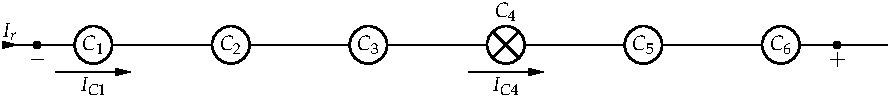
\includegraphics[scale=0.7]{../Figuras/AsociacionSerieCelulas}
    \par\end{center}


\end{frame}

\begin{frame}
  \frametitle{Punto caliente}

  \begin{center}
    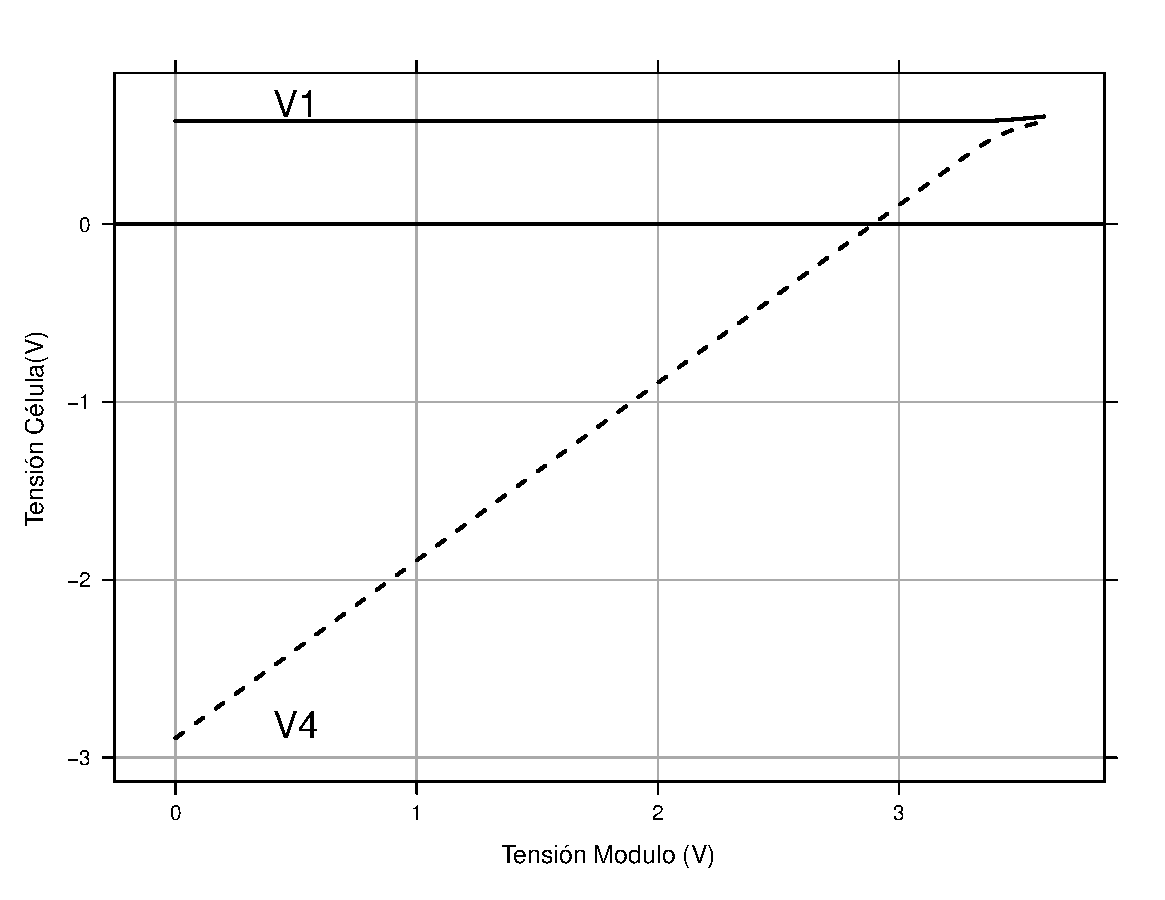
\includegraphics[scale=0.49]{../Figuras/TensionCelula_Sombras}
    \par\end{center}


\end{frame}

\begin{frame}
  \frametitle{Punto caliente}

  \begin{center}
    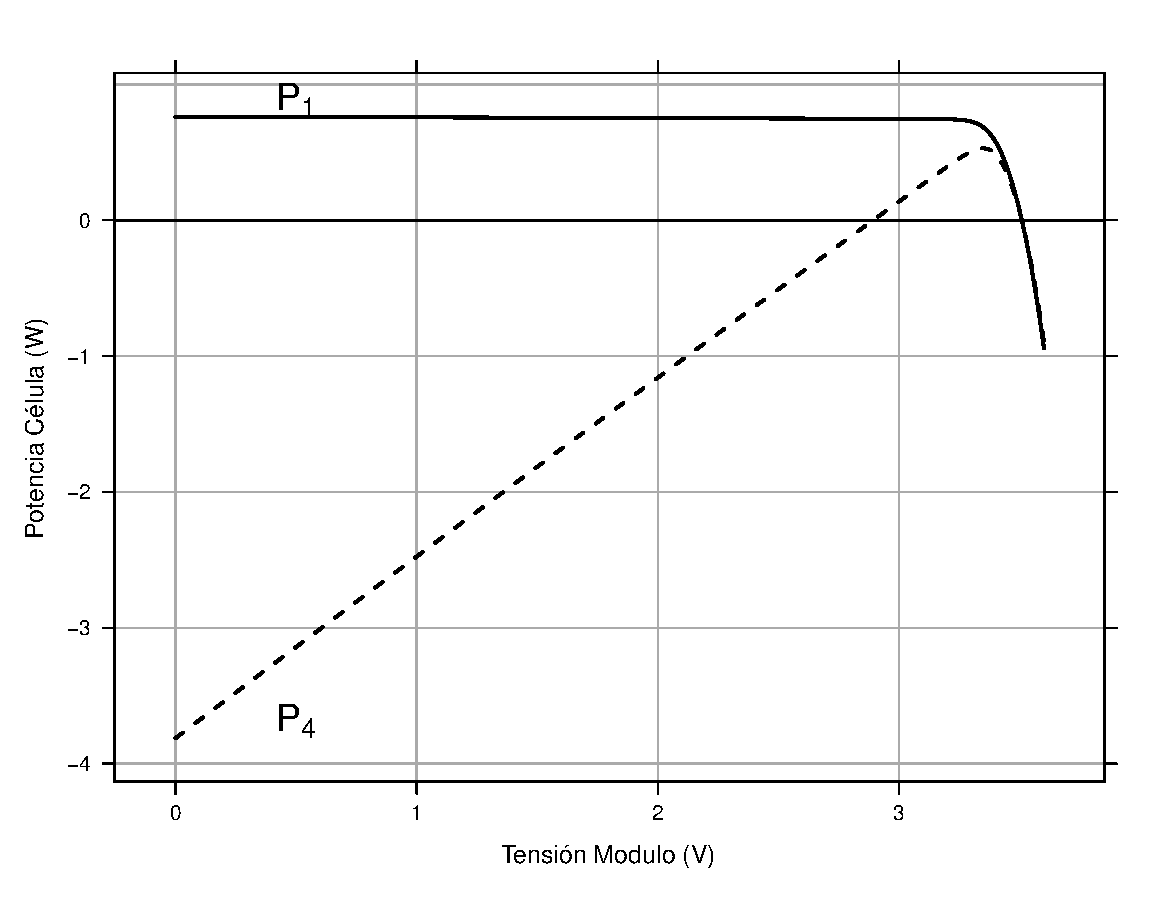
\includegraphics[scale=0.49]{../Figuras/PotenciaCelula_Sombra}
    \par\end{center}


\end{frame}

\begin{frame}
  \frametitle{Diodo de paso}

  \begin{center}
    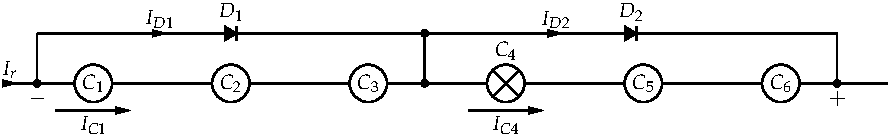
\includegraphics[scale=0.75]{../Figuras/AsociacionSerieCelulas_DiodosPaso}
    \par\end{center}


\end{frame}

\begin{frame}
  \frametitle{Curvas I-V con diodo de paso}

  \begin{center}
    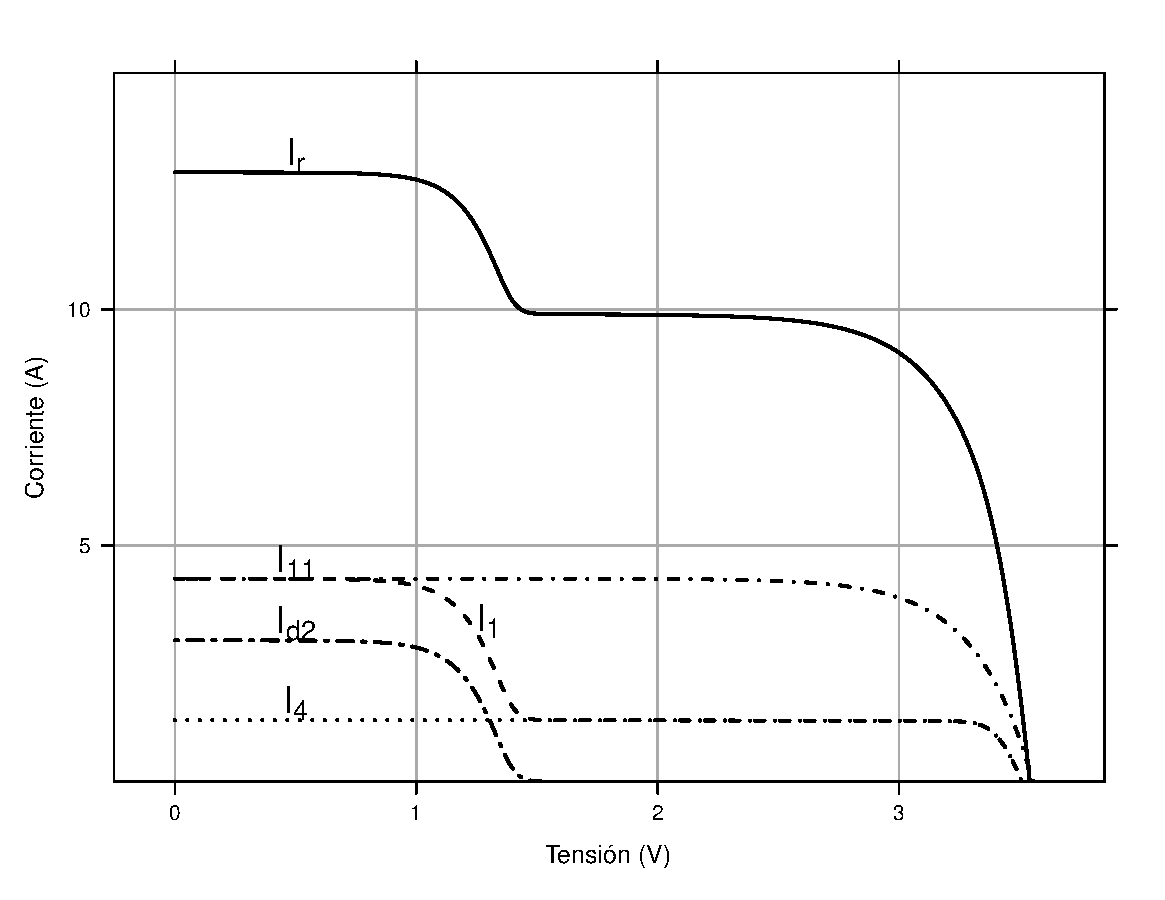
\includegraphics[scale=0.49]{../Figuras/CurvaIV_DiodoPaso}
    \par\end{center}


\end{frame}

\begin{frame}
  \frametitle{Tensión con diodo de paso}

  \begin{center}
    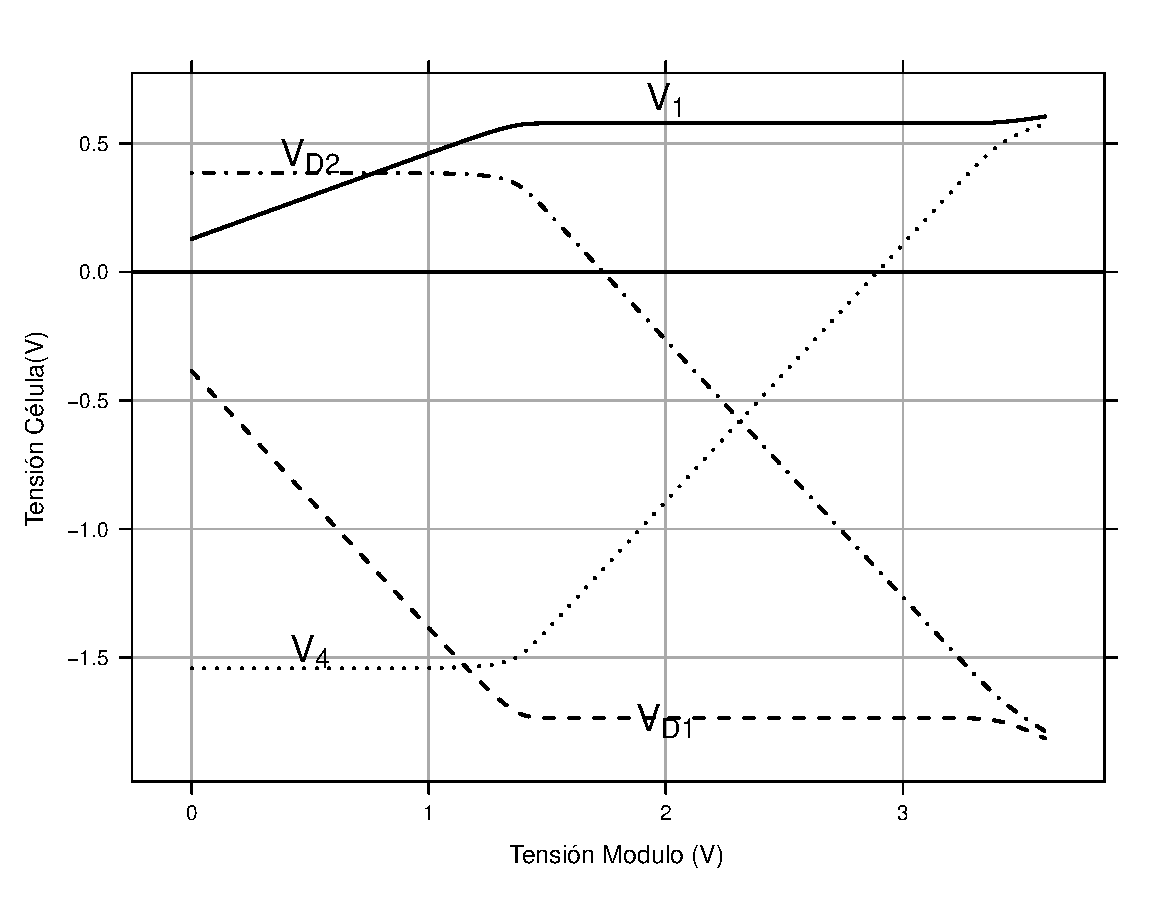
\includegraphics[scale=0.49]{../Figuras/TensionesCelulasDiodos_DiodoPaso}
    \par\end{center}


\end{frame}

\begin{frame}
  \frametitle{Curvas Potencia con diodo de paso}

  \begin{center}
    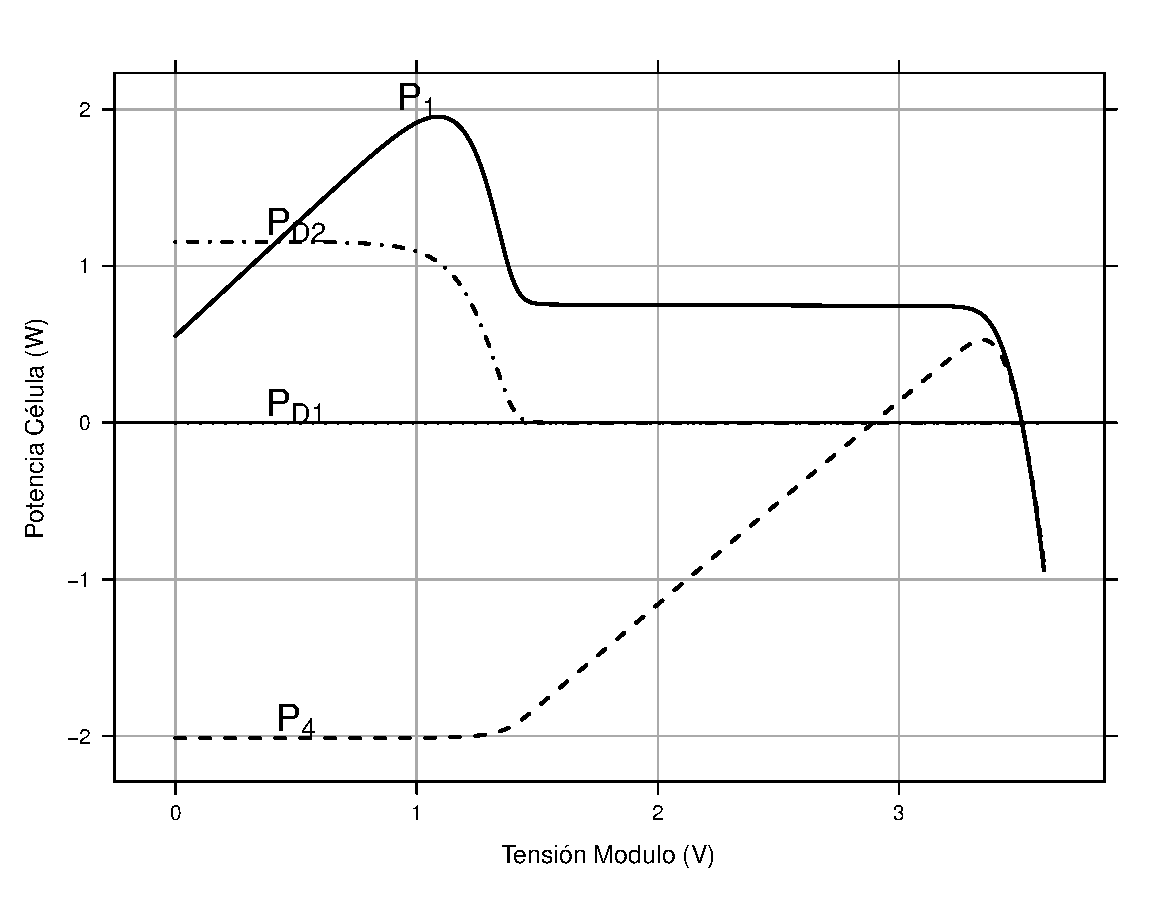
\includegraphics[scale=0.49]{../Figuras/PotenciaCelulas_DiodoPaso}
    \par\end{center}


\end{frame}

\begin{frame}
  \frametitle{Curva Módulo con Diodos de Paso}

  \begin{center}
    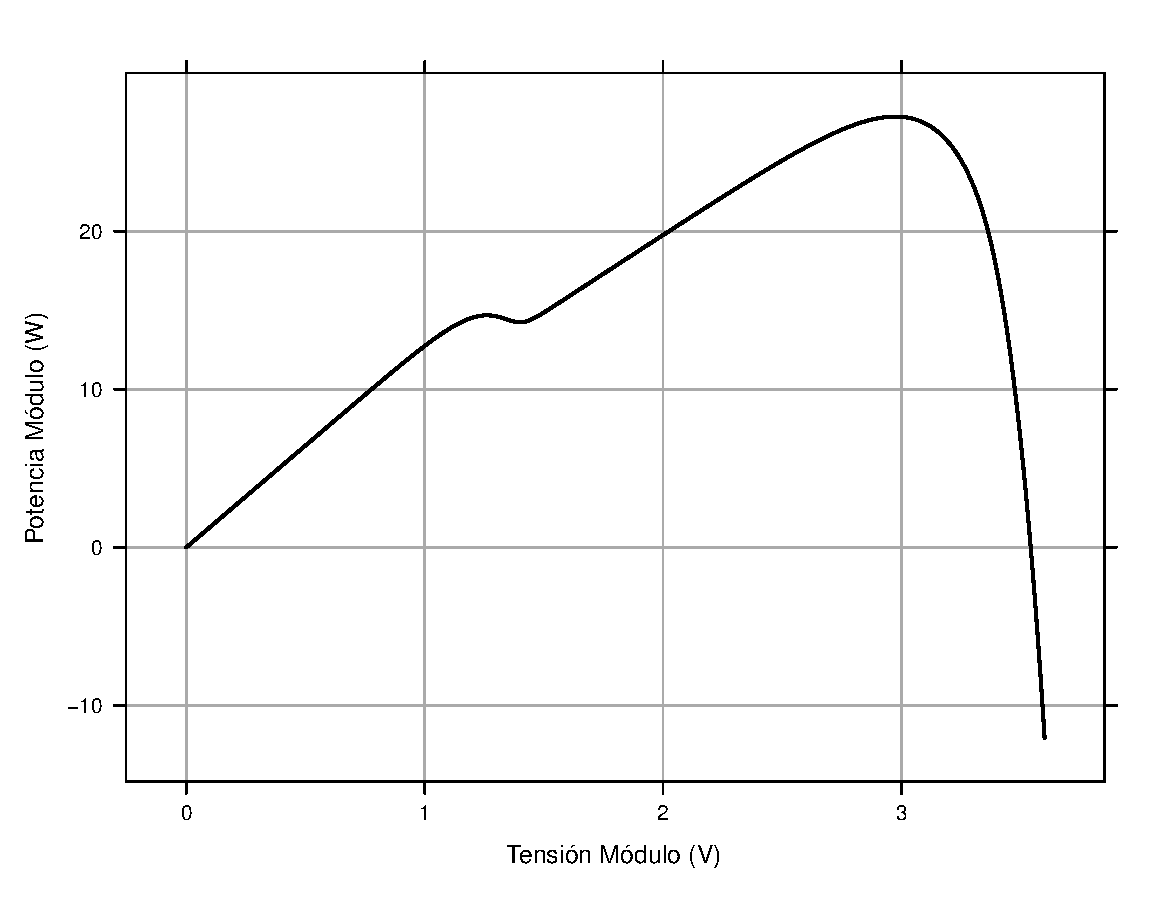
\includegraphics[scale=0.49]{../Figuras/PotenciaModulo}
    \par\end{center}


\end{frame}

\begin{frame}
  \frametitle{Diodos de paso}

  \begin{center}
    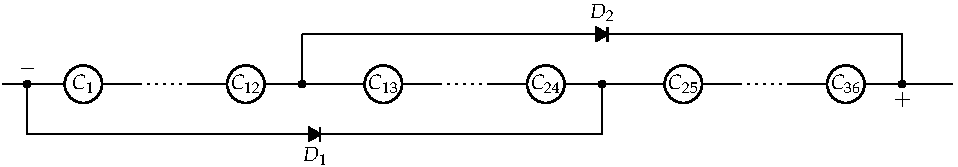
\includegraphics[scale=0.7]{../Figuras/AsociacionSerieCelulas_DiodosPasoAlternos}
    \par\end{center}

\end{frame}

\section{Generador Fotovoltaico}


\subsection{Definición}

\begin{frame}
  \frametitle{Generador Fotovoltaico}
  \begin{itemize}
  \item Un generador fotovoltaico es una asociación eléctrica de
    módulos fotovoltaicos para adaptarse a las condiciones de
    funcionamiento de una aplicación determinada.
  \item Se compone de un total de $N_{p}\cdot N_{s}$ módulos, siendo
    $N_{p}$ el número de ramas y $N_{s}$ el número de módulos en cada
    serie.
  \item El número de ramas define la corriente total del generador y
    el número de modulos por serie define la tensión del generador.
  \end{itemize}

\end{frame}

\begin{frame}
  \frametitle{Generador Fotovoltaico}

  \begin{center}
    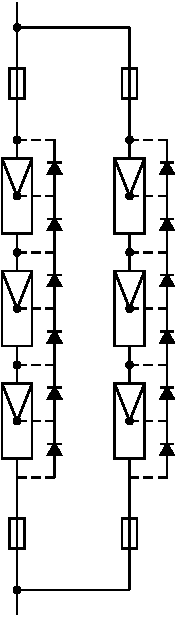
\includegraphics[angle=270]{../Figuras/AsociacionModulos}
    \par\end{center}
\end{frame}

\subsection{Pérdidas por dispersión}


\begin{frame}
  \frametitle{Pérdidas por dispersión}

\begin{block}{}
  Los parámetros eléctricos de un módulo FV presentan dispersión: la
  producción energética será menor que la ideal.
\end{block}

\end{frame}

\begin{frame}
  \frametitle{Pérdidas por dispersión}

\begin{block}{}
  La corriente de máxima potencia de un conjunto de módulos puede
  caracterizarse por una distribución tipo Weibull\[
  f(I_{mpp})=\alpha\beta^{-\alpha}I_{mpp}^{\alpha-1}exp\left[-\left(\frac{I_{mpp}}{\beta}\right)^{\alpha}\right]\]
  siendo $\alpha$ el factor de forma y $\beta$ el factor de escala de
  la distribución. La eficiencia de conexión serie es:\[
  \eta_{cs}=\frac{I_{mpp}^{r}}{\overline{I_{mpp}}}\] siendo
  $I_{mpp}^{r}$ la corriente de la rama, y $\overline{I_{mpp}}$ la
  media de las corrientes del grupo de módulos.

\end{block}

\end{frame}

\begin{frame}
  \frametitle{Pérdidas por dispersión}
  \begin{itemize}
  \item A partir de la distribución y la definición de eficiencia de
    conexión serie puede deducirse que ésta se calcula mediante\[
    \eta_{cs}=N^{-\frac{1}{\alpha}}\] siendo N el número de módulos en
    la serie. Por tanto, \textbf{la eficiencia disminuye si aumenta
      N}. Asimismo, la eficiencia aumenta con $\alpha$.
  \item Por otra parte, puede demostrarse que la \textbf{tensión de un
      grupo de módulos} puede modelarse mediante una función
    \textbf{gaussiana} y que \textbf{la dispersión de valores de
      tensión es suficientemente baja para poder considerar que la
      eficiencia de conexión de ramas en paralelo es igual a 1.}
  \end{itemize}

\end{frame}

\begin{frame}
  \frametitle{Pérdidas por dispersión}
  \begin{itemize}
  \item La dispersión de un conjunto depende inversamente del valor de
    $\alpha$, así que un \textbf{método para reducir las pérdidas por
      dispersión} consiste en \textbf{realizar clasificaciones} de los
    módulos atendiendo a sus valores reales de corriente.
  \item En sistemas de cierta entidad, puede ser conveniente realizar
    una clasificación en tres categorías y crear cada rama con módulos
    de una misma categoría.
  \item Este método puede suponer reducciones del 2-3\% en las
    pérdidas globales del sistema.
  \end{itemize}

\end{frame}

\begin{frame}
  \frametitle{Pérdidas por dispersión}
  \begin{block}{Problema}
    \begin{itemize}
    \item Las clasificaciones se realizan en base a las médidas
      realizadas por los fabricantes con``flash''.
    \item \textbf{La indeterminación asociada a este método en
        relación a las medidas a sol real son del mismo rango que la
        separación entre categorías.}
    \end{itemize}
  \end{block}
\end{frame}

\section{Ejemplos de generadores fotovoltaicos}




\begin{frame}[plain]
  \frametitle{}

  \noindent \begin{center}
    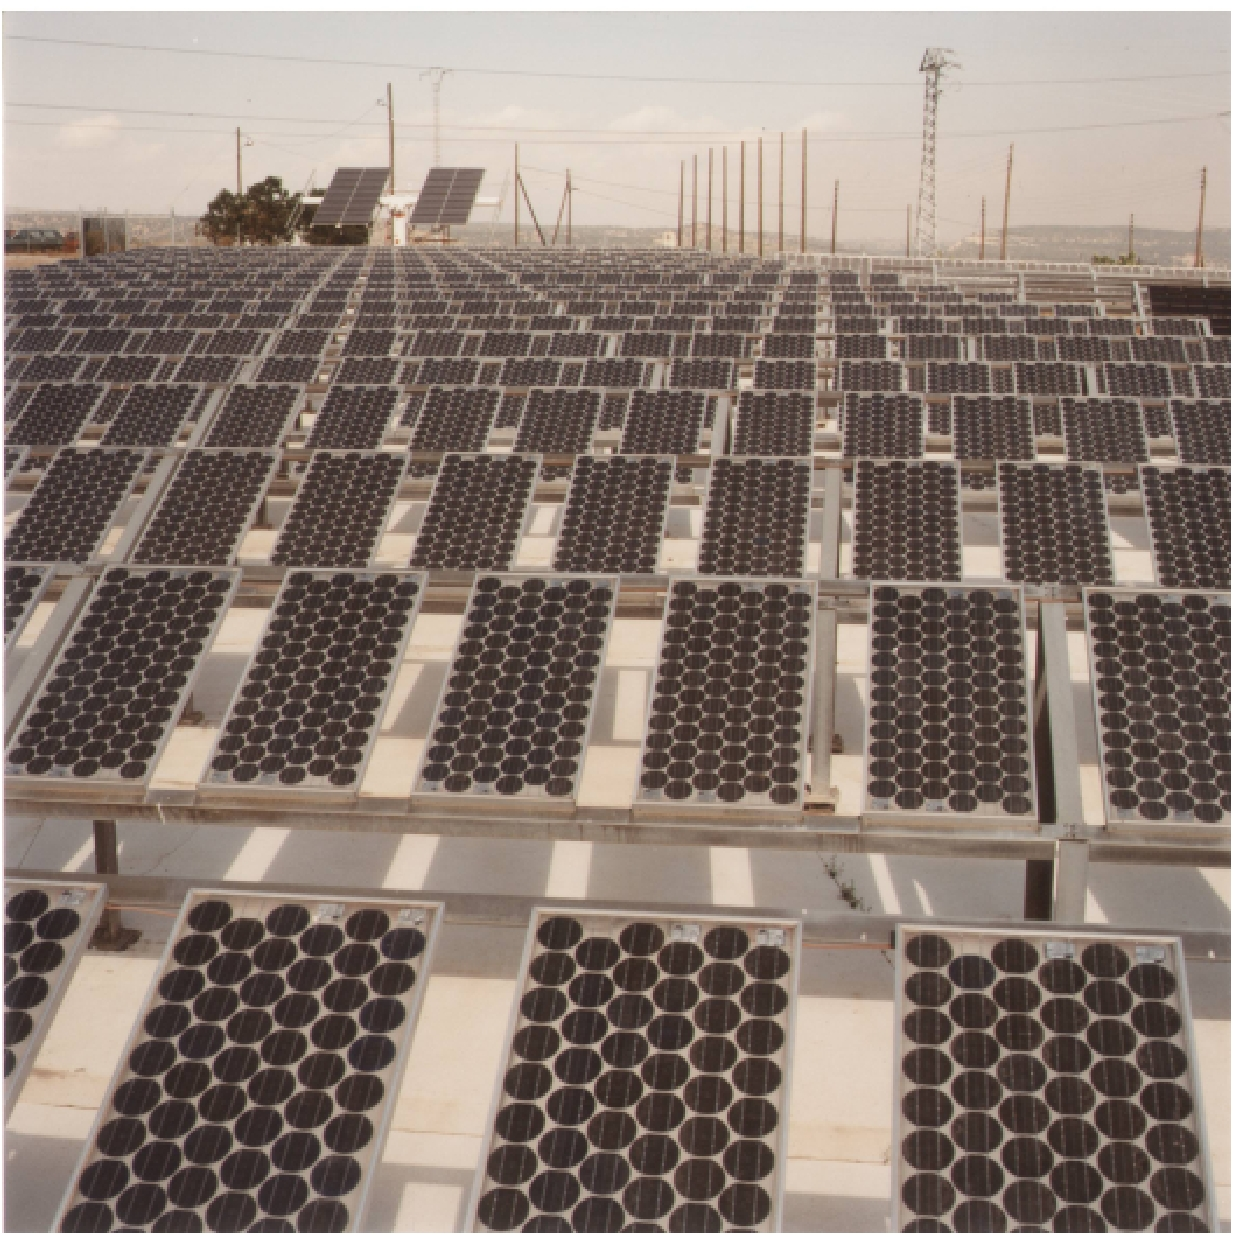
\includegraphics[scale=1.5]{../Fotos/Bifacial.jpg}
    \par\end{center}


\end{frame}

\begin{frame}[plain]
  \frametitle{}

  \noindent \begin{center}
    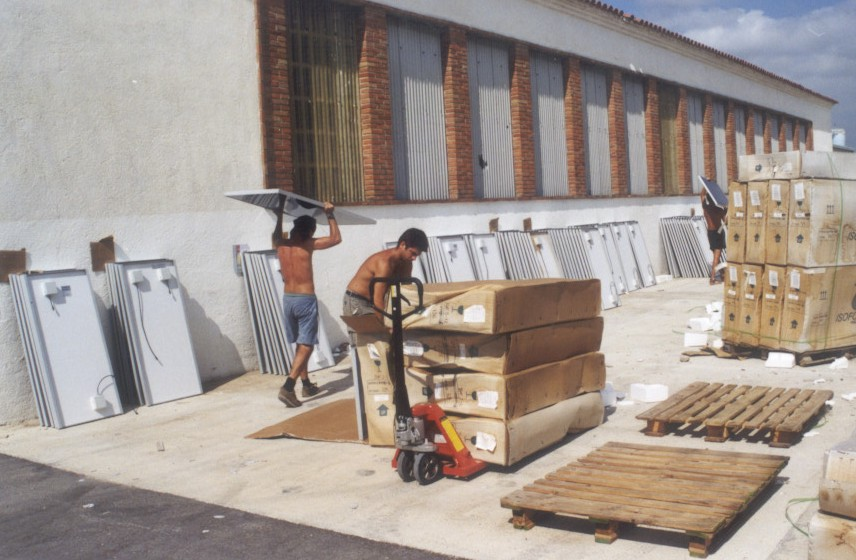
\includegraphics[scale=0.8]{../Fotos/clasificacion2.jpg}
    \par\end{center}


\end{frame}

\begin{frame}[plain]
  \frametitle{}

  \noindent \begin{center}
    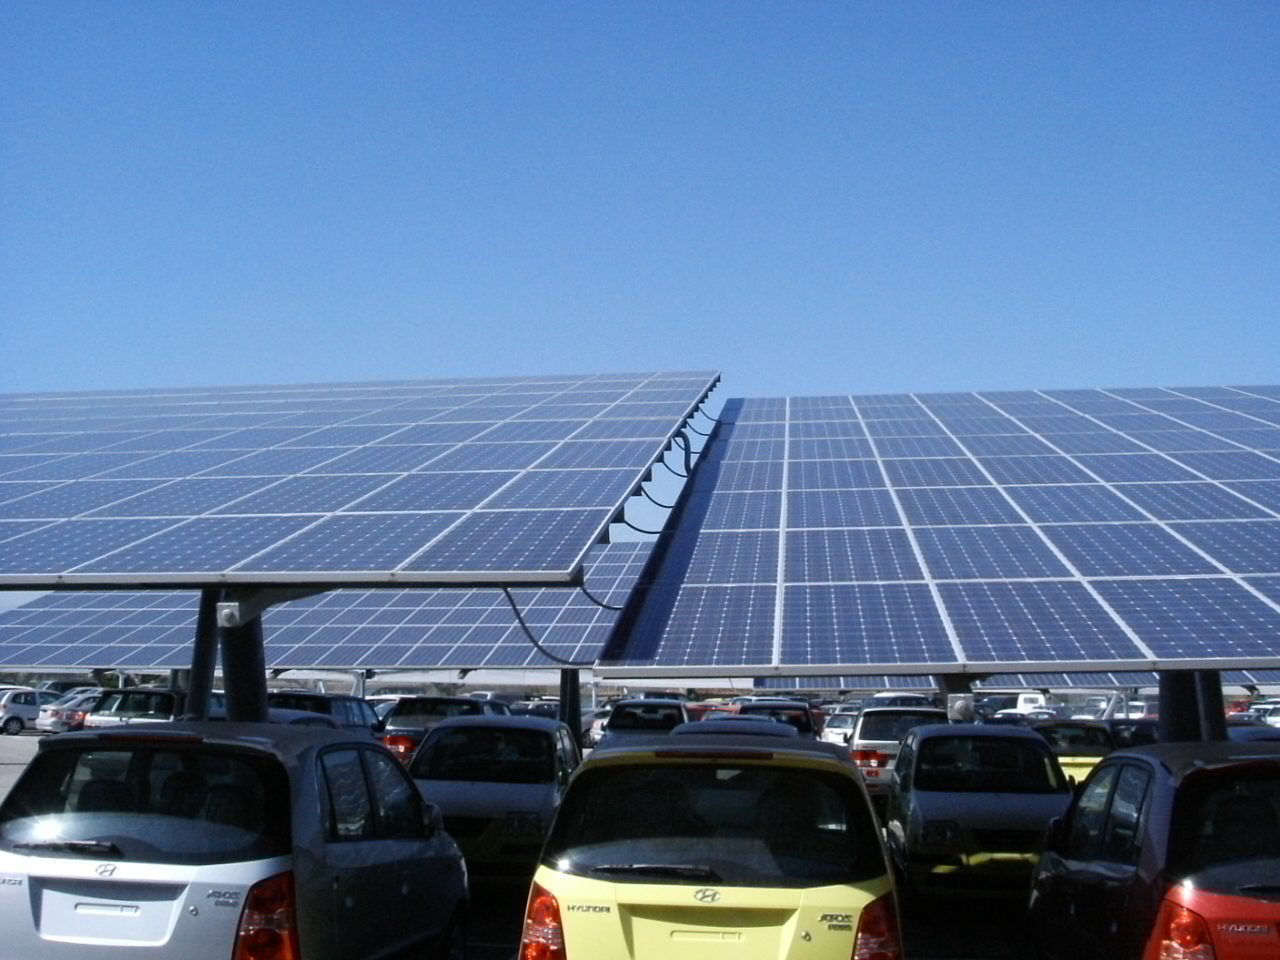
\includegraphics[scale=0.25]{../Fotos/dscf0997.jpg}
    \par\end{center}


\end{frame}

\begin{frame}[plain]
  \frametitle{}

  \noindent \begin{center}
    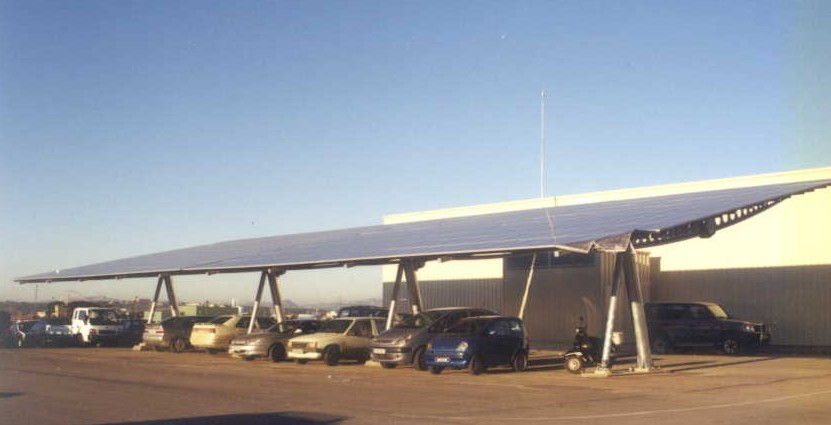
\includegraphics[scale=0.8]{../Fotos/ModulosRotos.jpg}
    \par\end{center}


\end{frame}

\begin{frame}[plain]
  \frametitle{}

  \noindent \begin{center}
    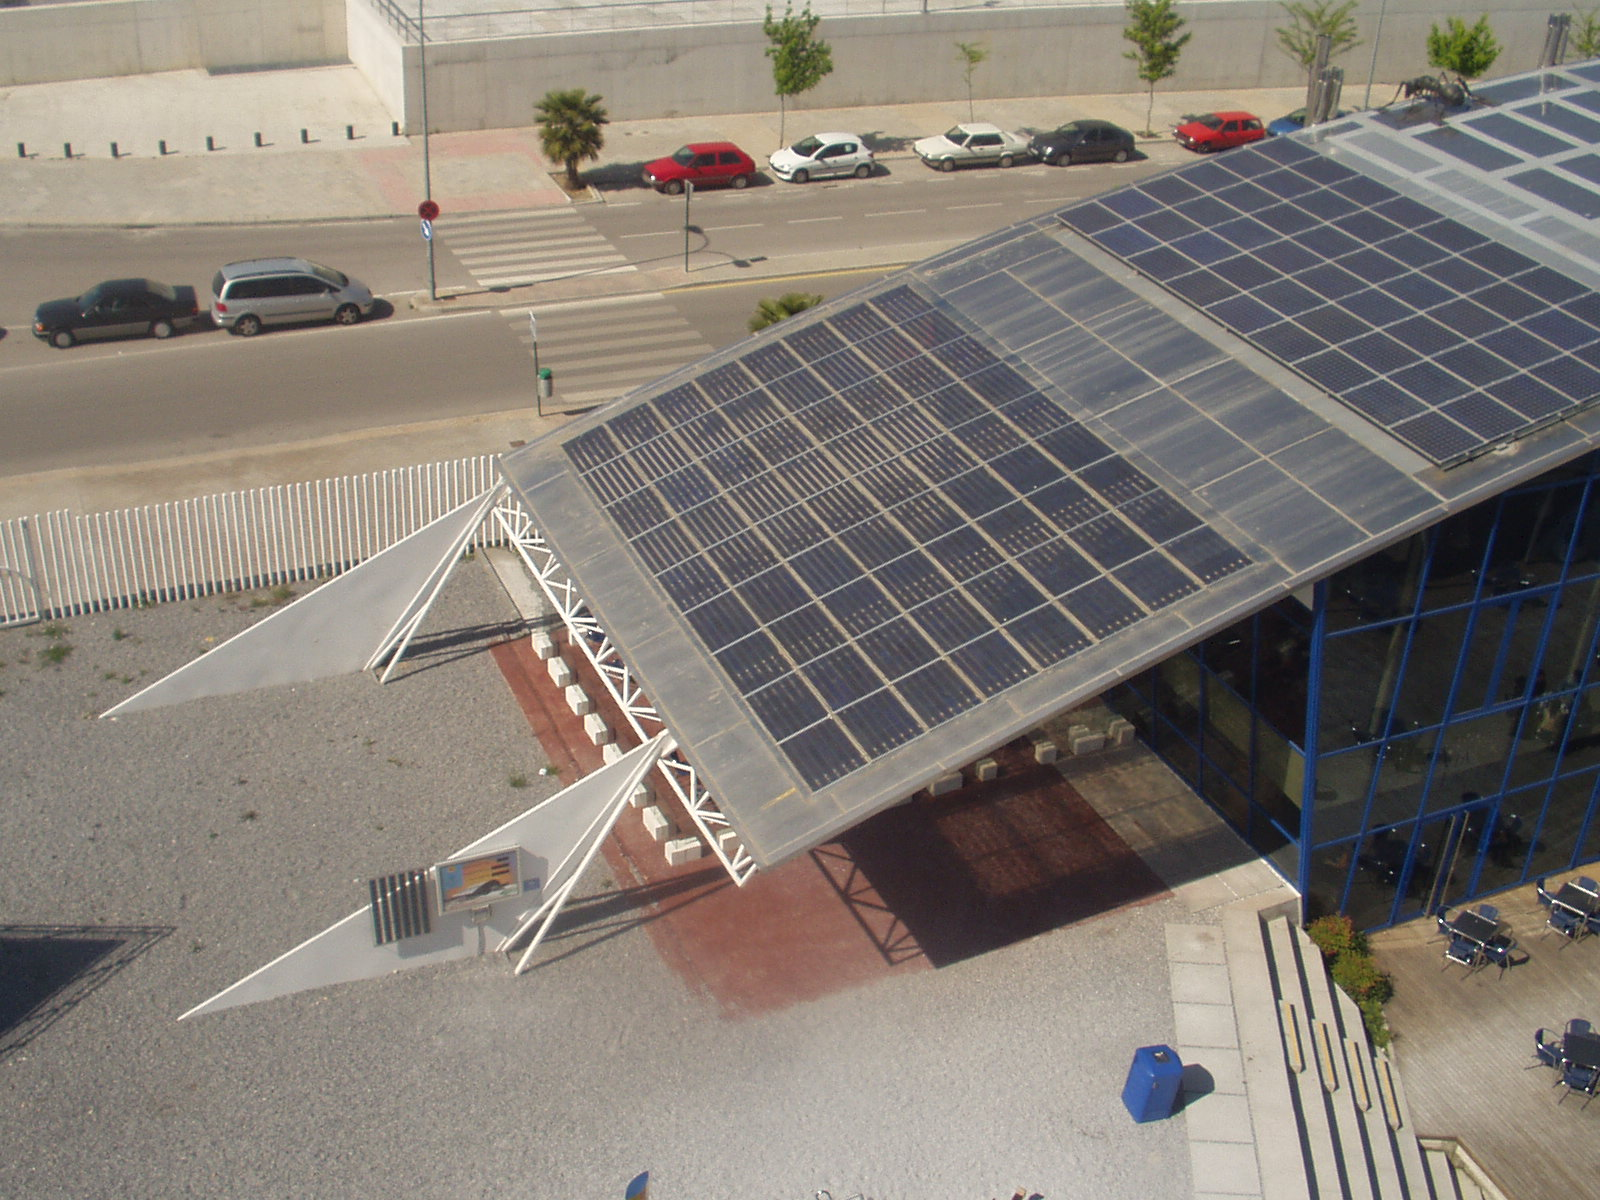
\includegraphics[scale=0.2]{../Fotos/p1010007.jpg}
    \par\end{center}


\end{frame}

% \begin{frame}[plain]
%   \frametitle{}

%   \noindent \begin{center}
%     \includegraphics[scale=0.1]{../Fotos/pb200764.jpg}
%     \par\end{center}


% \end{frame}

\begin{frame}[plain]
  \frametitle{}

  \noindent \begin{center}
    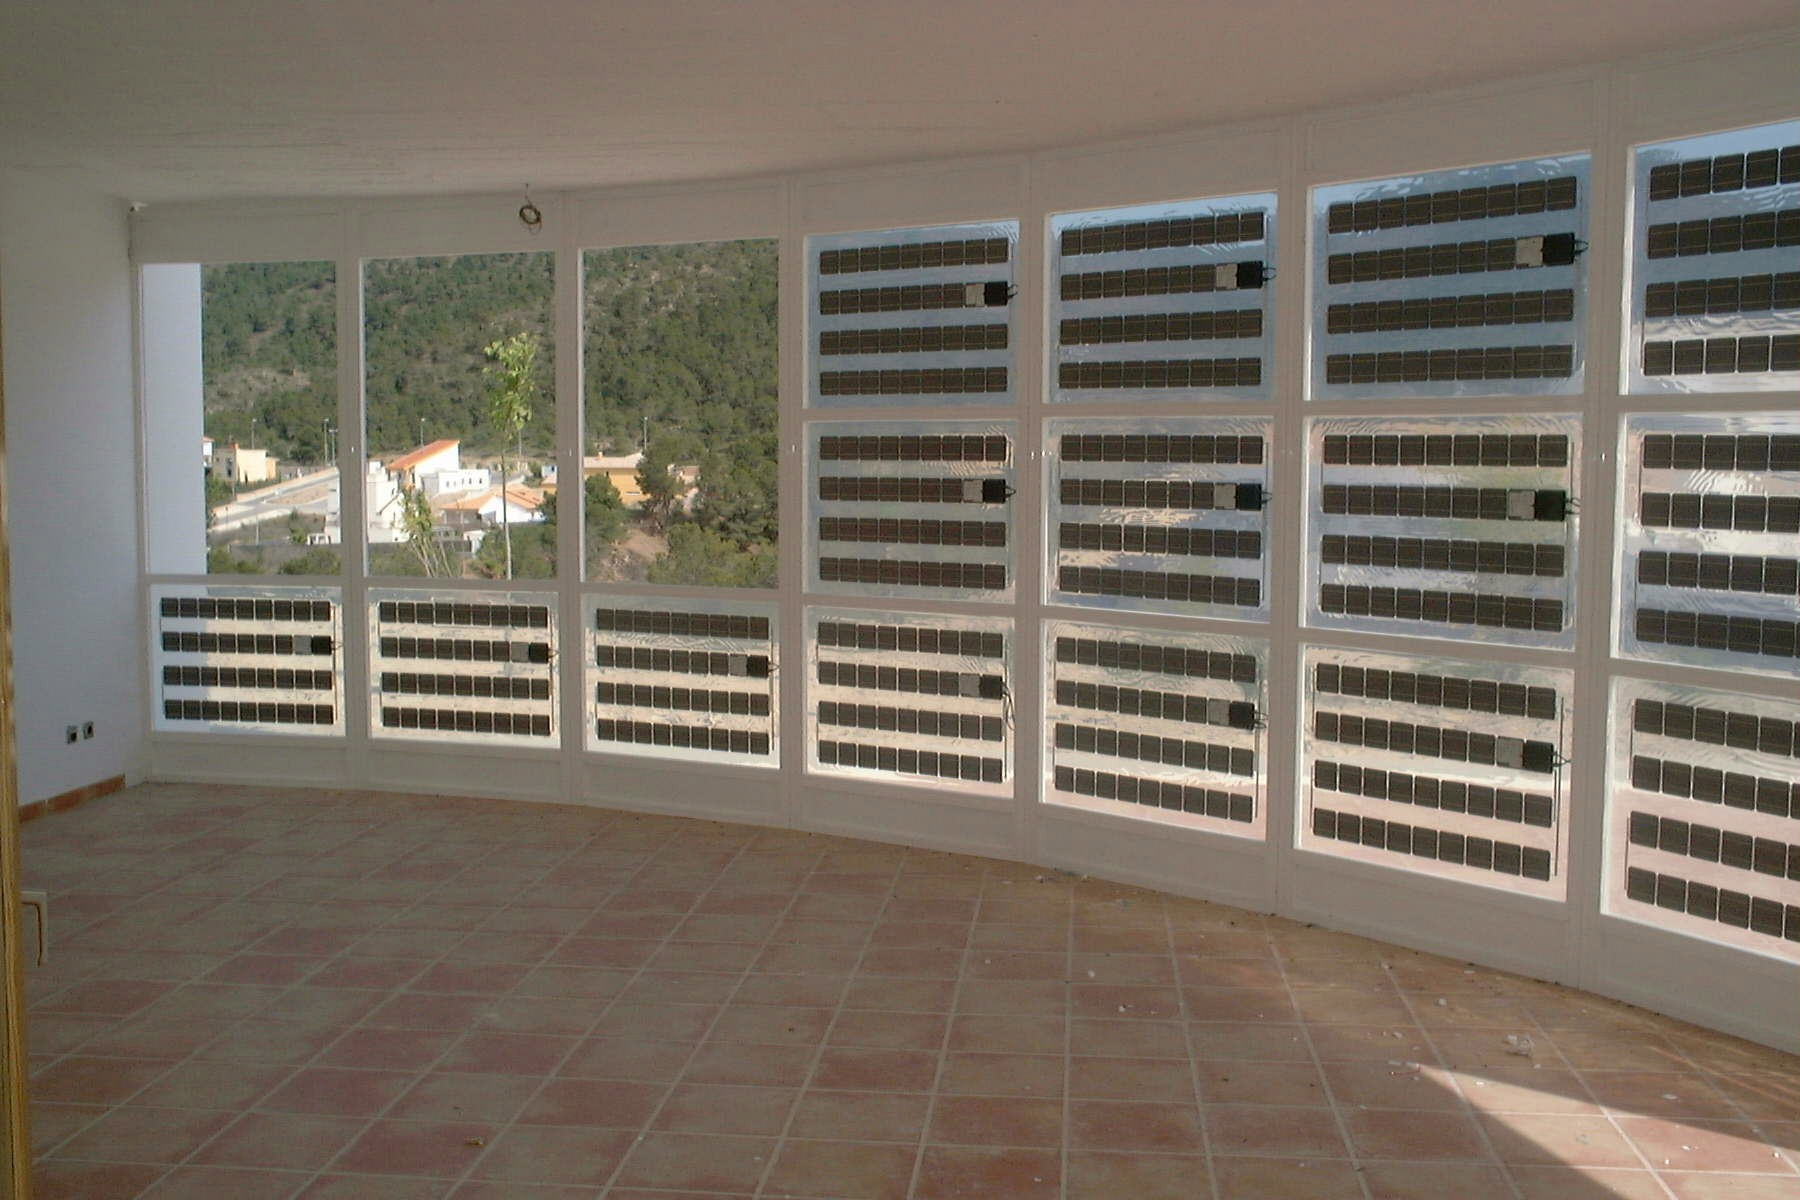
\includegraphics[scale=0.7]{../Fotos/TorreguilInterior2.jpg}
    \par\end{center}


\end{frame}

\begin{frame}[plain]
  \frametitle{}

  \noindent \begin{center}
    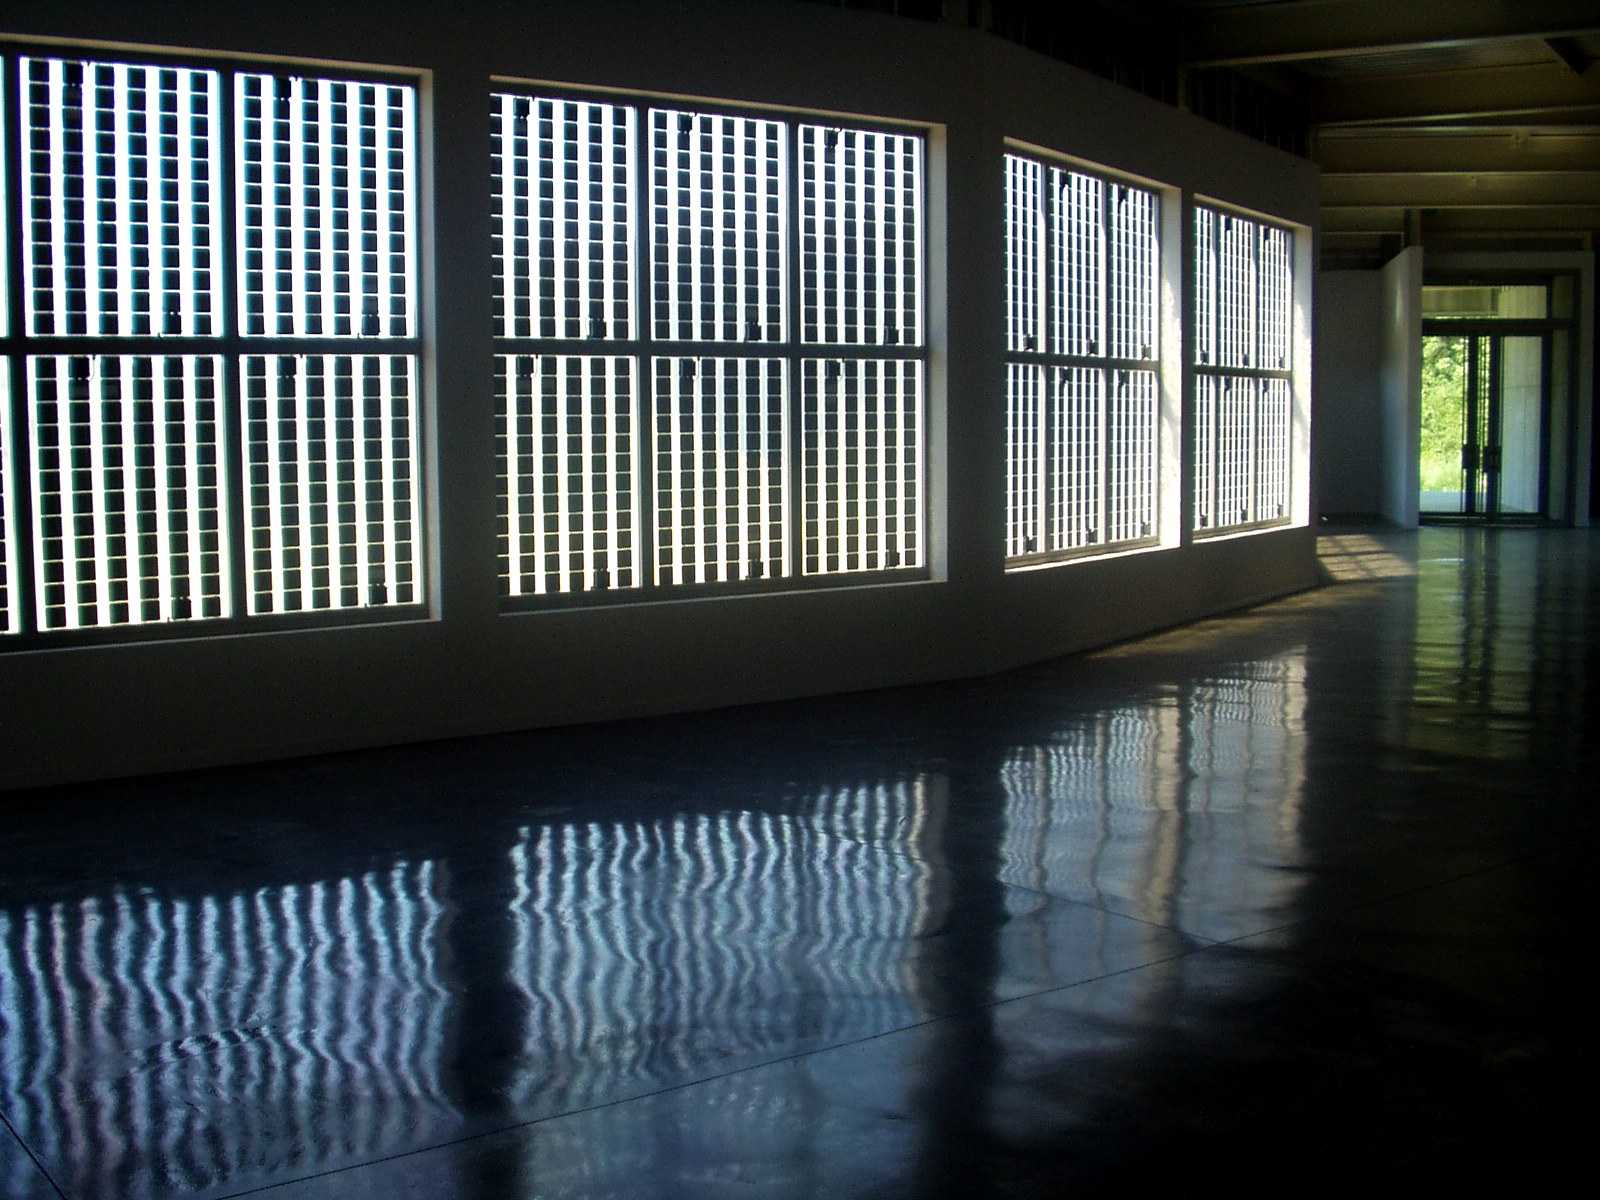
\includegraphics[scale=0.2]{../Fotos/VistadesdeInterior.jpg}
    \par\end{center}


\end{frame}

\end{document}
